\chapter{Retrieval-Augmented Generation}
I Large Language Models sono uno strumento estremamente potente e versatile. Tuttavia, possiedono anche numerose limitazioni e difetti che possono renderli inaffidabili in alcune situazioni o inadatti per determinati compiti. Inoltre, la loro conoscenza è limitata a quanto appreso durante la fase di addestramento, e le loro funzionalità si concentrano principalmente sulla generazione di testo. Per superare queste limitazioni sono stati sviluppati diversi accorgimenti che spaziano dal semplice Prompt Engineering al Fine Tuning, fino alla progettazione di architetture più complesse in grado di integrare capacità di ragionamento all'interno del modello.
Nello sviluppo del progetto presentato in questa tesi, sono state impiegate molte di queste tecniche (vedi Capitolo \ref{cap:omnibot1}), con un focus particolare su un approccio basato su un'architettura denominata Retrieval-Augmented Generation.

\section{Cos'è RAG?}
Retrieval-Augmented Generation (RAG) \cite{whatisrag,raghandbook,gao2024retrievalaugmentedgenerationlargelanguage} è un'architettura che combina tecniche di Information Retrieval (IR) con tecniche di Natural Language Generation (NLG) per generare risposte più accurate e coerenti. L'idea alla base di RAG è quella di integrare un modulo di retrieval all'interno di un LLM per fornire ad esso informazioni aggiuntive e contestuali durante la fase di generazione del testo. In questo modo, il modello può accedere a una vasta quantità di conoscenza esterna e utilizzarla per migliorare la qualità delle risposte generate.

Il funzionamento della versione elementare di RAG è abbastanza semplice e consiste in due fasi principali:
\begin{enumerate}
    \item \textbf{Retrieval}: In questa fase, l'LLM utilizza un modulo di retrieval (retriever) per recuperare i documenti rilevanti da una base di conoscenza esterna (knowledge base). Il retriever può essere progettato in diversi modi, ma in generale, il suo compito principale è quello di identificare i documenti che contengono le informazioni necessarie per rispondere alla domanda posta.
    \item \textbf{Generation}: Una volta recuperati i documenti rilevanti, il modello utilizza le informazioni contenute in essi per generare una risposta accurata e coerente. Il generatore può essere un qualsiasi LLM pre-addestrato.
\end{enumerate}

\section{Come funziona RAG?}
\begin{figure}[!t]
    \centering
    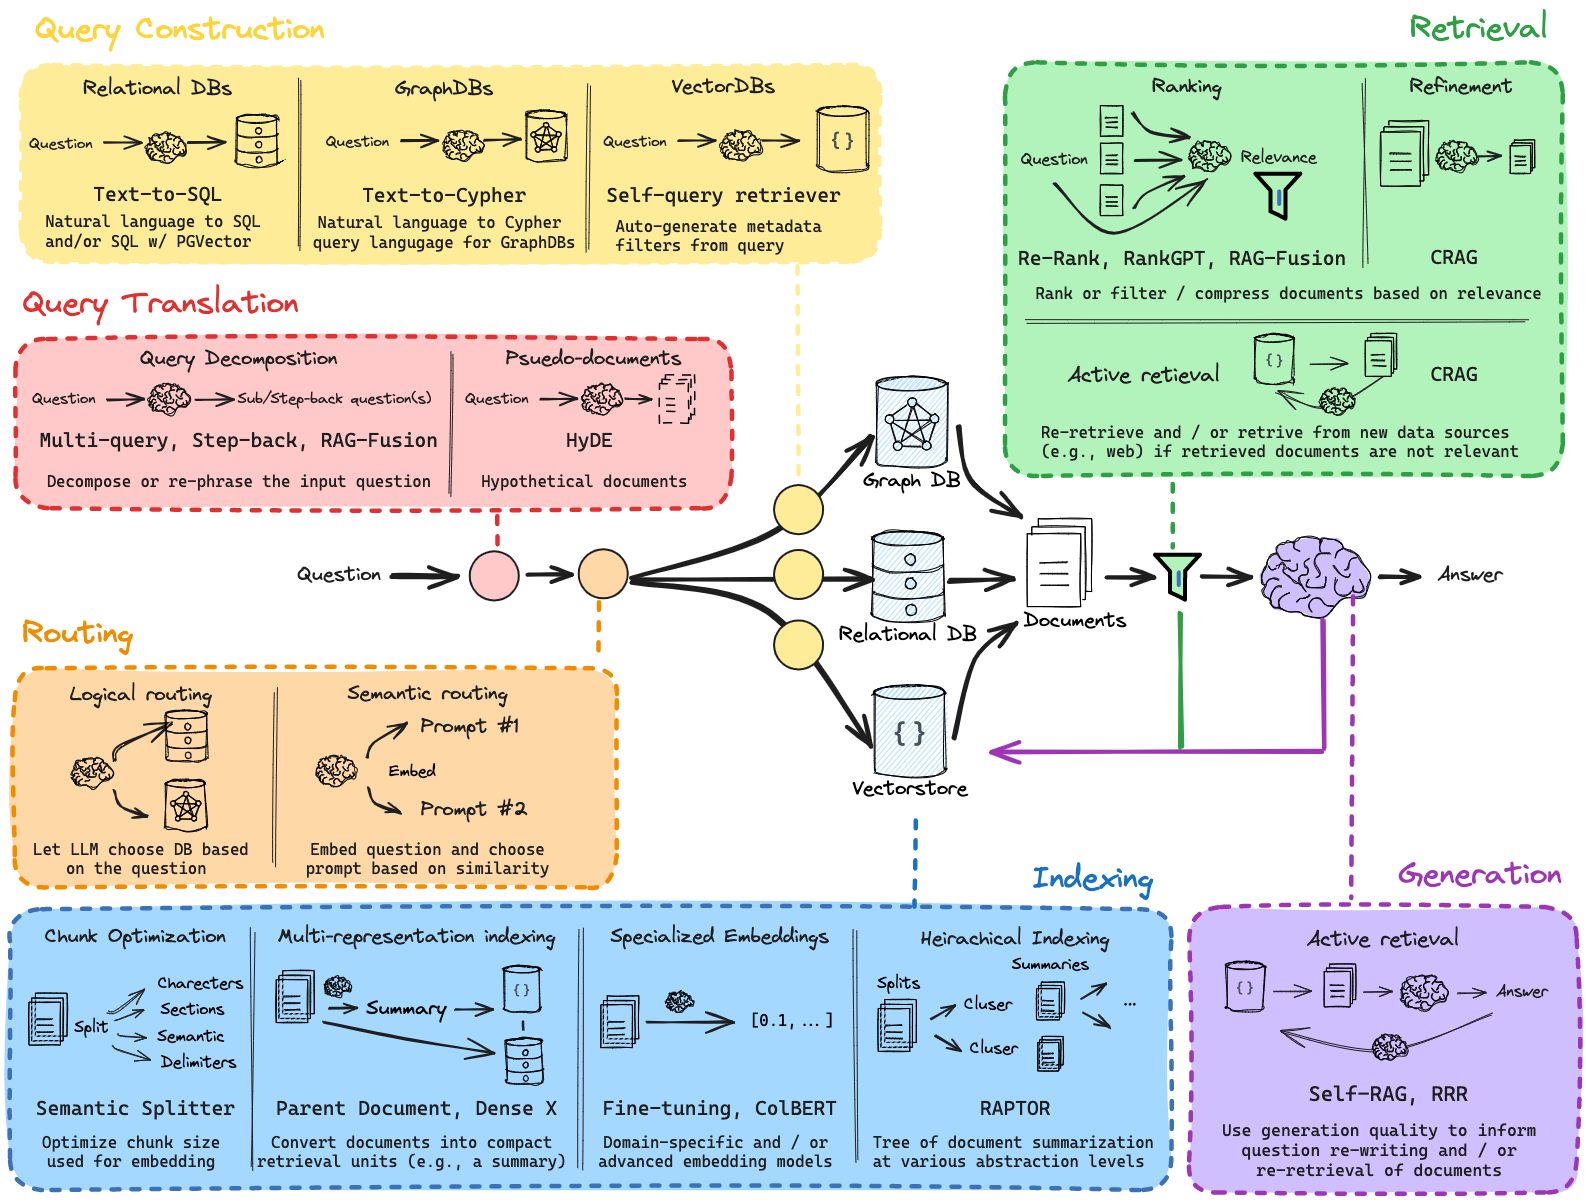
\includegraphics[width=\textwidth]{Images/cap2/rag_workflow.png}
    \caption{Workflow di RAG \cite{ragworkflow}}
    \label{fig:rag_workflow}
\end{figure}
RAG è un'architettura altamente personalizzabile e flessibile che può essere adattata a diversi compiti e scenari, quindi, nonostante il suo funzionamento di base rimanga lo stesso in tutte le sue varianti, la sua implementazione pratica può variare notevolmente a seconda delle esigenze specifiche.

\subsection{RAG passo dopo passo}
Analizziamo ora il funzionamento di RAG passo dopo passo (vedi \figurename{~\ref{fig:rag_workflow}}):

\subsubsection{Indexing}
Questa fase è presente in tutte le implementazioni di RAG e si tratta di una procedura che viene eseguita prima dell'avvio dell'architettura stessa. Serve a caricare i documenti della knowledge base all'interno di uno o più database in modo da renderli facilmente accessibili al retriever. Si può procedere in vari modi, ma solitamente si inizia effettuando un chunking dei dati e poi si procede con l'indicizzazione dei documenti. L'indicizzazione può essere fatta in maniera differente, a seconda del tipo di database utilizzato e a seconda dell'utilizzo che si deve fare dei documenti stessi. In particolare, per un database relazionale, si utilizza un'indicizzazione basata su chiavi primarie e chiavi esterne, mentre per un database vettoriale (vedi Paragrafo \ref{subsec:database_vettoriale}) si utilizza un'indicizzazione basata su vettori di embeddings. In aggiunta, è possibile utilizzare tecniche di indicizzazione più avanzate, come quella basata su grafi (ad esempio tramite Neo4j \cite{neo4j}) per ottenere implementazioni più efficienti e performanti. Quest'ultima tipologia è molto utile quando si vuole creare un sistema di indici gerarchici, vale a dire, un sistema in cui i documenti sono organizzati in una struttura ad albero o grafo che permette di accedere velocemente a documenti simili o correlati \cite{forer2024inferringscientificcrossdocumentcoreference}.

\subsubsection{Query Translation}
Si tratta della prima fase di elaborazione dell'input, ma non sempre viene implementato. Quando questo modulo viene utilizzato, la query dell'utente viene tradotta in una equivalente nel significato ma più adatta per il retriever. Questo passaggio è particolarmente utile quando il linguaggio utilizzato dal modello è diverso da quello della knowledge base. Ad esempio, se esso è addestrato in inglese ma la knowledge base è in italiano, la query dell'utente deve essere tradotta in inglese prima di essere passata al retriever. In questo passo è anche possibile che la query venga suddivisa in sotto-queries più specifiche per migliorare la precisione del retriever e per permettere al modello di rispondere a domande più complesse.

\subsubsection{Routing}
Il modulo di routing è responsabile della selezione del retriever più adatto per la query in ingresso. In generale, un sistema RAG può utilizzare diversi retriever, ognuno specializzato in un determinato tipo di query o di knowledge base. Il modulo di routing si occupa di identificare il retriever più adatto per la query in ingresso e di passare la query a tale retriever per il recupero dei documenti rilevanti. Questo modulo si occupa anche di decidere quale prompt utilizzare per il generatore in base ai risultati del retriever o alla natura della query. Ovviamente, il routing può essere implementato in modi diversi a seconda delle esigenze specifiche del sistema ma non è necessario se il sistema utilizza un solo retriever o se la gestione dei prompt è delegata ad un altro modulo o non è, anch'essa, necessaria.

\subsubsection{Query Construction}
Questa fase è presente in tutte le implementazioni di RAG e consiste nella costruzione della query da passare al retriever. La query può essere costruita in diversi modi a seconda delle esigenze specifiche del sistema, ma in generale, deve essere progettata in modo da massimizzare la precisione e la completezza del recupero dei documenti rilevanti. Inoltre, la query deve essere progettata in modo da massimizzare la coerenza e la coesione del testo generato dal modello. Si deve tenere presente che i documenti che verranno recuperati dal retriever si trovano dentro database di vario tipo, come database vettoriali, database relazionali, database di grafi, ecc. e quindi la query costruita deve essere compatibile con il tipo di database utilizzato.

\subsubsection{Retrieval}
È la fase cardine di RAG e consiste nel recupero effettivo dei documenti. Il retriever utilizza la query costruita nella fase precedente per recuperare i documenti rilevanti dalla knowledge base. Le informazioni recuperate possono essere di molteplici tipologie, da dati testuali (articoli, libri, pagine web, codice, ecc.) a contenuti multimediali (audio, foto, video ecc.). Il modo in cui recupera i documenti dipende dal tipo di database utilizzato e a seguito del recupero, i documenti possono essere restituiti integralmente al modello o subire ulteriori elaborazioni. Ad esempio, i documenti possono essere filtrati, ordinati, aggregati, ecc. prima di essere passati al generatore \cite{liu2023lostmiddlelanguagemodels}.

\subsubsection{Generation}
La fase finale consiste nell'elaborazione da parte della rete dei dati ricevuti in input (prompt di sistema, query dell'utente, documenti recuperati, ecc.) per generare la risposta finale. Il generatore può essere un qualsiasi LLM pre-addestrato, ma può anche essere un modello addestrato specificamente per il compito di generazione di testo. Il generatore utilizza le informazioni contenute nei documenti recuperati per generare una risposta accurata e coerente alla query dell'utente. La risposta generata può essere di vario tipo, da un semplice testo a una tabella, un grafico, un'immagine, ecc. Spesso è conveniente utilizzare varianti di LLM di tipo IT (Instruction Tuning) \cite{zhang2024instructiontuninglargelanguage,ouyang2022traininglanguagemodelsfollow} poiché riescono a generare risposte strutturate e più coerenti quando rispondono a domande basate su istruzioni specifiche ("Spiega perché...", "Riassumi questo...", "Traduci questa frase...").
Recenti studi hanno evidenziato che l'utilizzo di modelli LLM di piccole dimensioni \cite{hsieh2023distillingstepbystepoutperforminglarger,mukherjee2023orcaprogressivelearningcomplex} all'interno di architetture RAG può portare ad avere un sistema più rapido ma al tempo stesso molto accurato e coerente (ad esempio FLARE \cite{jiang2023activeretrievalaugmentedgeneration}).

\subsection{Database Vettoriale}
\label{subsec:database_vettoriale}
Per la realizzazione del progetto, che verrà introdotto nel Capitolo \ref{cap:omnibot1}, è stato utilizzato un database vettoriale per memorizzare i documenti della knowledge base. Un database vettoriale (detto anche VectorStore) memorizza i dati sotto forma di vettori, dove ogni documento o dato non strutturato è rappresentato tramite un embedding, ovvero un vettore di numeri reali.

Gli embeddings sono ottenuti tramite tecniche di machine learning che trasformano testi, immagini o audio in rappresentazioni numeriche dense, catturando così la semantica o le caratteristiche salienti dei dati.
Questa tipologia di database è particolarmente adatta per gestire dati non strutturati, poiché consente di effettuare operazioni di recupero e ricerca basate sulla similarità tra vettori. In un sistema del genere, il retriever può confrontare rapidamente la query dell'utente con i documenti presenti nella knowledge base, restituendo quelli più rilevanti grazie alla vicinanza tra i rispettivi embeddings nello spazio vettoriale.

Nella versione più recente del progetto, gli embeddings sono stati ottenuti utilizzando un modello di tipo Sentence Transformer dell'azienda Cohere. Questo, denominato \textit{"embed-multilingual-v3.0"} \cite{cohereembed} è stato addestrato su un corpus di testi molto ampio e diversificato, in modo da catturare le relazioni semantiche tra le parole e i concetti. Gli embeddings generati da questo embedder hanno dimensione 1024 e sono in grado di catturare le relazioni semantiche tra i documenti in modo efficace e accurato.
Quindi, appena un documento viene caricato nel database vettoriale, le sue features più significative vengono codificate in un vettore di dimensione 1024 che rappresenta il documento nello spazio vettoriale. Si può visualizzare lo spazio vettoriale come un'astrazione matematica in cui i documenti sono rappresentati come punti e la distanza tra i punti rappresenta la similarità tra i documenti. In questo modo, il retriever può confrontare la query dell'utente con i documenti presenti nel database e restituire quelli più rilevanti in base alla vicinanza tra i rispettivi embeddings.

\subsubsection{Visualizzazione di uno Spazio Vettoriale}
Per poter visualizzare graficamente i documenti nello spazio vettoriale, è possibile utilizzare tecniche di riduzione della dimensionalità, come la Principal Component Analysis (PCA) \cite{MACKIEWICZ1993303} o la t-Distributed Stochastic Neighbor Embedding (t-SNE) \cite{cai2022theoreticalfoundationstsnevisualizing,roy2024trustworthydimensionalityreduction}, che proiettano i vettori in uno spazio a dimensioni ridotte (ad esempio bidimensionale o tridimensionale), permettendo di visualizzare i documenti in un grafico.
Questo tipo di visualizzazione è particolarmente utile per capire come i documenti sono distribuiti nello spazio vettoriale e per identificare eventuali cluster o pattern nascosti nei dati.

Nello specifico verrà utilizzata la tecnica t-SNE poiché è più adatta a visualizzare dati non lineari e a catturare le relazioni semantiche tra i documenti.
Quest'ultima trasforma le distanze in probabilità per preservare le relazioni locali e utilizza una distribuzione t di Student per ridurre la dimensionalità in modo non lineare. In questo caso, la preservazione delle relazioni locali, porta a mantenere i punti vicini nei dati originali vicini anche nel nuovo spazio ridotto.
Si tratta di un approccio più diretto rispetto a quello della PCA che trovando le direzioni (componenti principali) lungo le quali i dati variano di più, riduce la dimensionalità mantenendo il più possibile la varianza originale dei dati.
Di seguito è riportato un frammento di codice Python che mostra come utilizzare la libreria scikit-learn per applicare la tecnica t-SNE \cite{scikittsne} a un insieme di vettori multidimensionali:
\begin{lstlisting}[label=lst:tsne, caption={Esempio applicazione t-SNE}]  
from sklearn.manifold import TSNE
from sklearn.preprocessing import LabelEncoder
from vectordb import VectorDatabase

vectorstore = VectorDatabase.load_from_local(*@\textcolor{functionyellow}{(}@*)"path/to/db"(*@\textcolor{functionyellow}{)}@*)
vectors = vectorstore.get_vectors(*@\textcolor{functionyellow}{()}@*)
labels = vectorstore.get_labels(*@\textcolor{functionyellow}{()}@*)

tsne = TSNE(*@\textcolor{functionyellow}{(}@*)n_components=(*@\textcolor{numberyellow}{3}@*), perplexity=(*@\textcolor{numberyellow}{50}@*)(*@\textcolor{functionyellow}{)}@*)
label_encoder = LabelEncoder(*@\textcolor{functionyellow}{()}@*)

vectors_3d = tsne.fit_transform(*@\textcolor{functionyellow}{(}@*)vectors(*@\textcolor{functionyellow}{)}@*)
encoded_labels = label_encoder.fit_transform(*@\textcolor{functionyellow}{(}@*)labels(*@\textcolor{functionyellow}{)}@*)

# (*@\textcolor{commentsgreen}{...}@*)
\end{lstlisting}
Una volta applicato l'algoritmo t-SNE, è possibile visualizzare i documenti nello spazio tridimensionale utilizzando una libreria di visualizzazione.
\begin{figure}[!t]
    \centering
    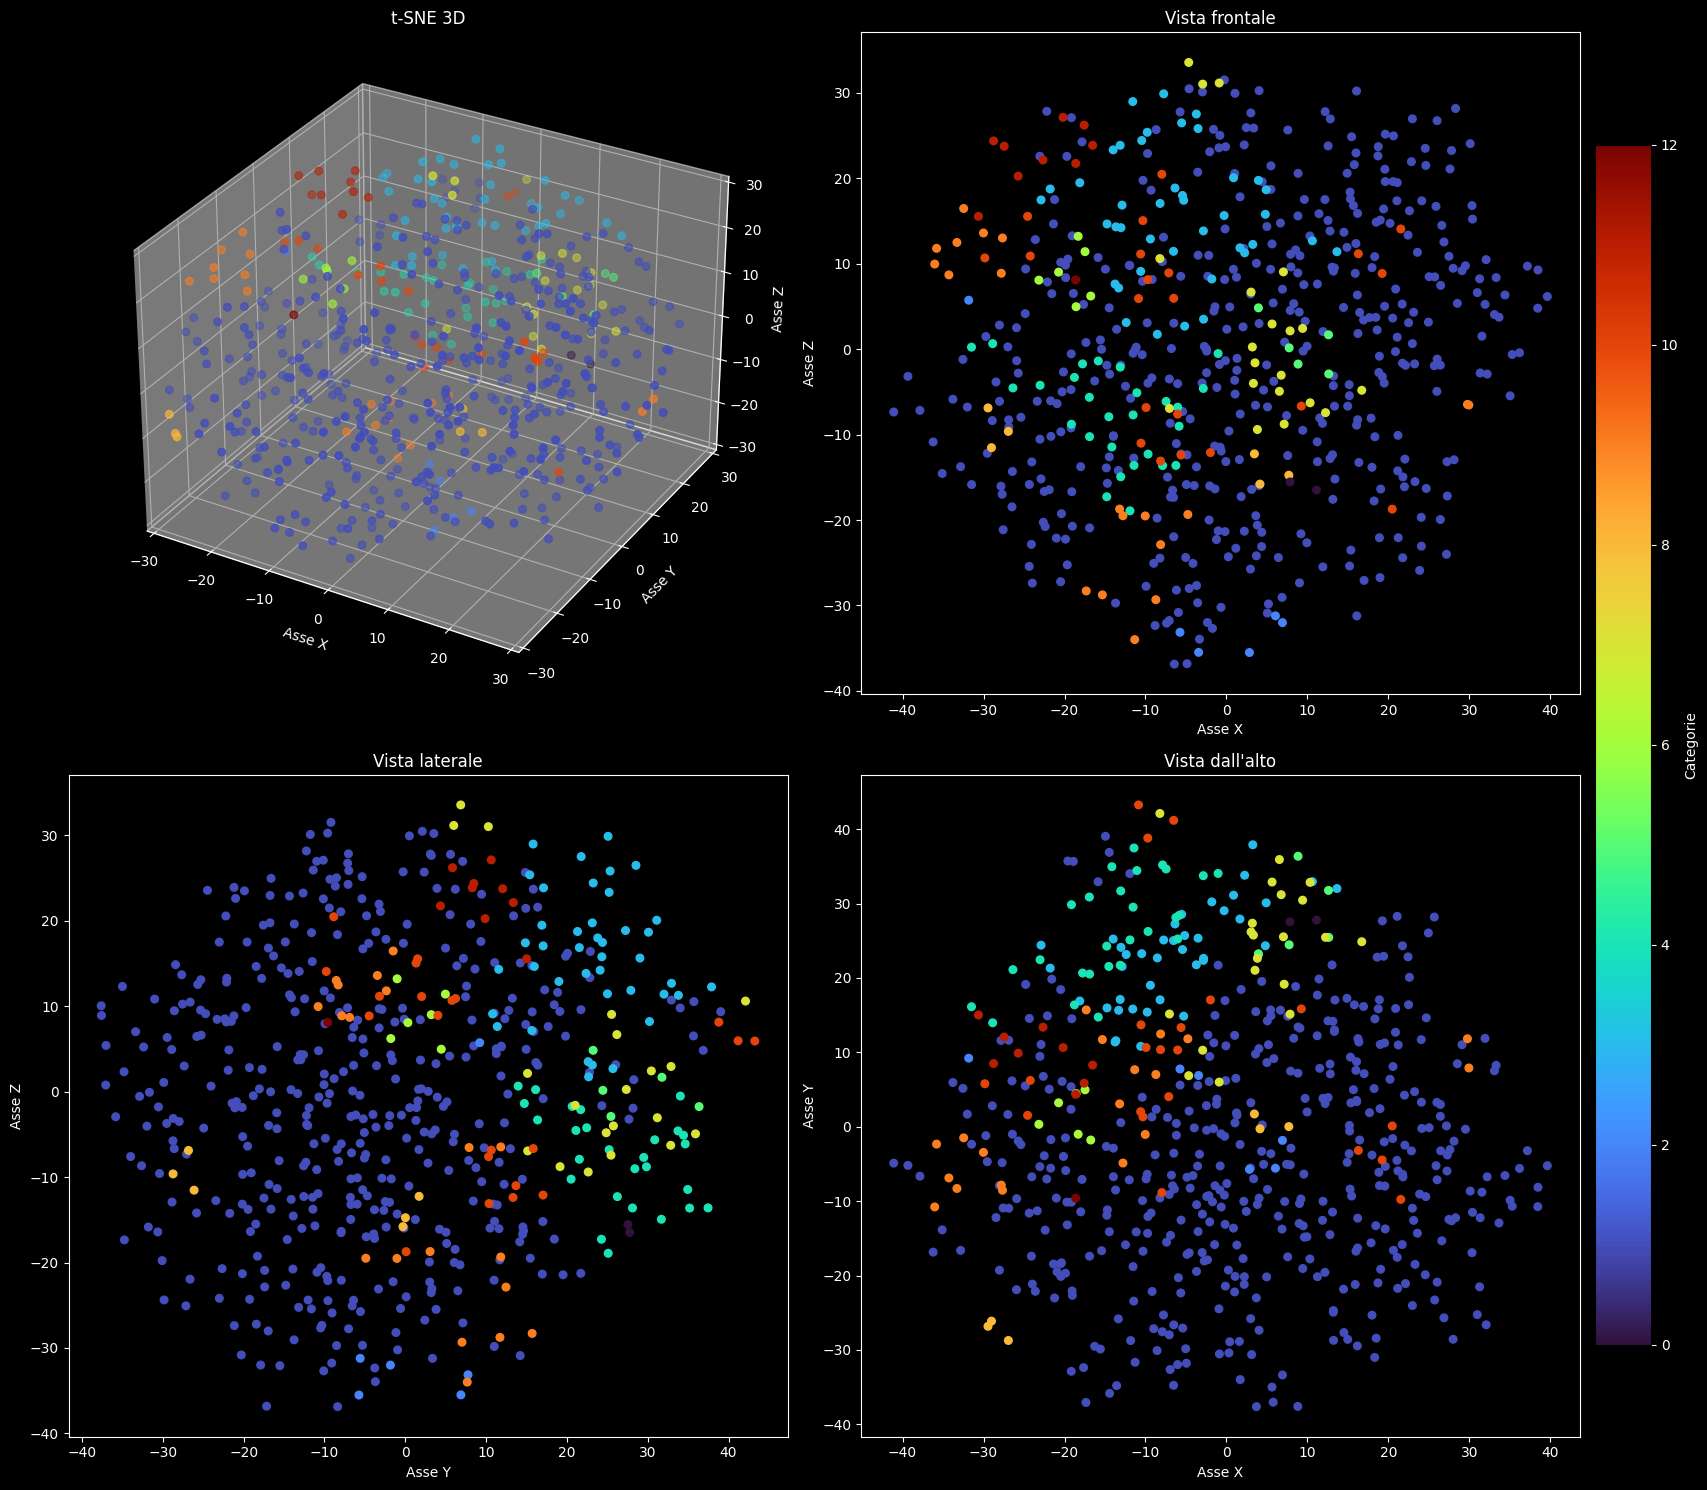
\includegraphics[width=\textwidth]{Images/cap2/nero.png}
    \caption{Visualizzazione di un database vettoriale tramite t-SNE}
    \label{fig:databse_vettoriale}
\end{figure}

Il grafico riportato in \figurename{~\ref{fig:databse_vettoriale}} è stato realizzato tramite la libreria Matplotlib e rappresenta tutti i documenti del database vettoriale come punti in uno spazio tridimensionale. Ogni punto ha un colore che è diverso a seconda della classe di appartenenza del documento stesso. Si può notare che molti punti dello stesso colore si riuniscono in aree ben distinte, suggerendo la presenza di cluster o gruppi di documenti simili tra loro. Più un punto è vicino ad un altro, più i due documenti corrispondenti sono simili tra loro. Naturalmente non è detto che punti vicini siano necessariamente dello stesso colore, infatti capita che documenti di classi differenti parlino di uno stesso argomento (anche se in modo diverso) e quindi siano vicini nello spazio vettoriale.
\subsection{Retriever Vettoriale}
Il retriever di un database vettoriale può essere implementato ed utilizzato in molti modi, il modo specifico in cui è stato implementato per il progetto presentato in questa tesi verrà introdotto a partire dal Capitolo \ref{cap:omnibot1}. In generale, un retriever vettoriale funziona confrontando la query dell'utente con i documenti presenti nel database e restituendo quelli più simili alla query in base alla vicinanza tra i rispettivi embeddings.

Dunque, per effettuare la ricerca, è prima necessario calcolare l'embedding della query dell'utente. Una volta fatto ciò si torna in output il documento, o meglio, una lista di documenti, più simili alla query. Si possono effettuare anche ricerche a partire da altri documenti stessi, in questo caso si calcola l'embedding del documento e si restituiscono i documenti più simili a quello in input.

Ci sono diverse tipologie di ricerche, le più comuni sono:
\begin{itemize}
    \item \textbf{Ricerca per similarità semantica}: Si cerca di trovare i documenti più simili alla query in base alla vicinanza tra i rispettivi embeddings.
    \item \textbf{Maximal Marginal Relevance (MMR)}: Si cerca di trovare i documenti più simili alla query ma che siano anche diversi tra loro. Questo approccio è utile per evitare la ripetizione di informazioni simili nei documenti restituiti.
\end{itemize}
Dopo ciascuna di queste ricerche è possibile applicare dei filtri di similarità o distanza che permettono di eliminare dall'output del retriever eventuali documenti non abbastanza simili alla query e quindi potenzialmente non rilevanti. Solitamente similarità o distanza vengono forniti tra i metadati dell'output del retriever (a seconda che la ricerca si basi sulla similarità o sulla distanza da embeddings noti) e assumono valori che vengono interpretati in maniera opposta: più è alto il valore di similarità (di solito tra 0 e 1), allora, più è basso il valore di distanza e viceversa. Solitamente la similarità si calcola utilizzando la \textit{Cosine Similarity}, mentre la distanza si calcola utilizzando la \textit{Euclidean Distance} o la \textit{Manhattan Distance}.
\begin{align}
    \text{Cosine Similarity} &= \frac{A \cdot B}{\|A\| \|B\|} \\
    \text{Euclidean Distance} &= \sqrt{\sum_{i=1}^{n} (A_i - B_i)^2} \\
    \text{Manhattan Distance} &= \sum_{i=1}^{n} |A_i - B_i|
\end{align}

\subsection{Tecniche di Prompt Engineering in RAG}
Il Prompt Engineering \cite{Beurer_Kellner_2023} è una tecnica che consiste nella progettazione di prompt specifici per guidare il modello nella generazione di testo. Questa tecnica è particolarmente utile quando si vuole controllare il comportamento dello stesso e indirizzarlo verso una determinata risposta. Nel contesto di RAG, il Prompt Engineering è utilizzato per guidare il generatore nella generazione di risposte accurate e coerenti, utilizzando le informazioni contenute nei documenti recuperati dal retriever. In un certo senso l'architettura RAG stessa è una forma di Prompt Engineering, poiché il retriever fornisce al generatore le informazioni necessarie per generare una risposta corretta. Praticamente l'LLM riceverà in input sia la query che la risposta ad essa. Tuttavia, è possibile utilizzare tecniche di Prompt Engineering più avanzate per migliorare ulteriormente le prestazioni del modello e per indirizzarlo verso risposte più precise. Ad esempio, si possono utilizzare prompt specifici per guidare il generatore nella generazione di risposte strutturate o per indirizzarlo verso risposte più lunghe e dettagliate. In particolare, si possono utilizzare prompt di sistema per fornire al modello informazioni aggiuntive sul contesto della conversazione o per guidarlo nella generazione di risposte di qualità superiore e maggiormente pertinenti.

Un esempio di prompt di sistema è il seguente:
\begin{lstlisting}[label=lst:prompt, caption={Esempio di prompt di sistema}, literate={.}{{\textcolor{stringbrown}{.}}}1 {,}{{\textcolor{stringbrown}{,}}}1 {=}{{\textcolor{white}{=}}}1]
RAG_PROMPT = (*@\textcolor{stringbrown}{"""Tu sei un assistente virtuale che aiuta}@*)
                (*@\textcolor{stringbrown}{gli utenti rispondendo alle loro domande.}@*)
                (*@\textcolor{stringbrown}{Rispondi nella stessa lingua della domanda.}@*)
                (*@\textcolor{stringbrown}{NON ripetere la domanda dell'utente.}@*)
                (*@\textcolor{stringbrown}{Rispondi con tono formale e professionale.}@*)
                (*@\textcolor{stringbrown}{Se non sai rispondere alla domanda, puoi}@*)
                (*@\textcolor{stringbrown}{dire "Non lo so".}@*)
                (*@\textcolor{stringbrown}{Puoi usare le informazioni contenute nei}@*)
                (*@\textcolor{stringbrown}{seguenti documenti:}@*)
                (*@\textcolor{defblue}{\{context\}}@*)
                
                (*@\textcolor{stringbrown}{Domanda:}@*)
                (*@\textcolor{defblue}{\{query\}}@*)(*@\textcolor{stringbrown}{"""}@*)
\end{lstlisting}
I campi \{context\} e \{query\} vengono riempiti con le informazioni recuperate dal retriever e con la query dell'utente, rispettivamente. In questo modo, il modello riceve in input tutte le informazioni necessarie per generare una risposta accurata e che sia compatibile con la domanda dell'utente. Inoltre, il prompt di sistema fornisce al generatore istruzioni dettagliate su come rispondere alla domanda e su come utilizzare le informazioni contenute nei documenti recuperati dal retriever.

\section{Perché RAG?}
RAG è uno strumento molto potente se integrato con un LLM, poiché permette di aggiungere conoscenze esterne migliorando la qualità delle risposte generate. Ma RAG è davvero la soluzione definitiva per risolvere tutte le limitazioni degli LLM? La risposta è no. Pur essendo efficace in molti contesti, ha alcuni difetti e limitazioni. In più, lo sviluppo di tecniche e modelli più sofisticati, insieme all'integrazione di framework all'avanguardia, sta lentamente spingendo RAG ai margini. Esaminiamo nel dettaglio le alternative e cerchiamo di rispondere alla domanda "Perché RAG?" in modo più approfondito.

\subsection{Alternative a RAG}
Esistono diverse metodologie per migliorare e personalizzare un modello linguistico, ciascuna con vantaggi e limitazioni specifiche. Tra queste, possiamo identificare:
\begin{itemize}
    \item \textbf{Fine Tuning}: Questa è una delle tecniche più comuni per personalizzare un LLM \cite{lu2024finetuninglargelanguagemodels}. Consiste nel riaddestrare il modello su un dataset specifico dopo l'addestramento originale, adattandone i parametri alle nuove esigenze.
        \begin{itemize}
            \item \textbf{Vantaggi}: Il modello diventa più accurato e specializzato per un determinato dominio.
            \item \textbf{Svantaggi}: Richiede elevate risorse computazionali e di tempo, oltre a grandi quantità di dati. È inoltre poco flessibile quando le informazioni devono essere aggiornate frequentemente.
        \end{itemize}
    \item \textbf{Instruction Tuning}: In questo caso, si adatta il comportamento del modello affinché segua meglio istruzioni in linguaggio naturale \cite{ouyang2022traininglanguagemodelsfollow}. Si basa sull'addestramento su compiti eterogenei, per migliorare la risposta a prompt strutturati sotto forma di istruzioni esplicite.
        \begin{itemize}
            \item \textbf{Vantaggi}: Migliora la capacità dell'LLM di affrontare diversi task attraverso prompt più complessi.
            \item \textbf{Svantaggi}: Sebbene ottimizzi le risposte, non aggiunge nuove informazioni e non risolve il problema dell'obsolescenza della conoscenza del modello.
        \end{itemize}
    \item \textbf{Prompt Tuning}: Questa tecnica si basa sull'ottimizzazione dei prompt per ottenere risposte migliori da un LLM pre-addestrato, senza modificarne i parametri interni. Il focus è sulla formulazione delle richieste in modo tale da sfruttare al massimo le conoscenze preesistenti del modello.
        \begin{itemize}
            \item \textbf{Vantaggi}: È computazionalmente efficiente, non richiede riaddestramento e può essere facilmente adattata a diversi contesti.
            \item \textbf{Svantaggi}: Non consente l'aggiunta di nuove informazioni, ma si limita a migliorare l'uso di quelle già presenti nel modello.
        \end{itemize}
    \item \textbf{LLM Agents}: Gli agenti basati su LLM estendono le capacità del modello linguistico con sistemi di esecuzione di task \cite{llmagents}. Questi agenti possono eseguire operazioni complesse, come navigare sul web o prendere decisioni basate su input dinamici.
        \begin{itemize}
            \item \textbf{Vantaggi}: Estendono l'applicabilità del prodotto oltre la generazione di testo, integrando capacità di esecuzione pratica.
            \item \textbf{Svantaggi}: Richiedono l'integrazione con sistemi complessi e, spesso, non sono orientati all'aggiunta di nuove conoscenze nel modello stesso.
        \end{itemize}
\end{itemize}

\subsection{RAG vs tutti}
RAG è la tecnica più adatta quando si vuole aggiornare la base di conoscenza di un LLM, senza richiedere un riaddestramento completo o un uso intensivo di risorse computazionali. A differenza delle altre tecniche, che mirano principalmente a modificare il comportamento del modello o a migliorare l'interazione con esso, RAG permette di integrare nuove informazioni esterne in modo dinamico \cite{ragandfine}.

Perché RAG? La risposta è semplice: è il metodo migliore per aggiungere informazioni nuove a un LLM senza la necessità di riaddestrarlo, offrendo così un aggiornamento della conoscenza in modo rapido ed efficiente. Tuttavia, non è la soluzione ideale per specializzare il modello o per fargli eseguire compiti complessi.
Il compromesso ottimale è l'integrazione di RAG con altre tecniche \cite{lewis2021retrievalaugmentedgenerationknowledgeintensivenlp,zhao2024retrievalaugmentedgenerationrag}. Ad esempio, una combinazione con agenti LLM o tecniche di modifica della catena di pensiero (chain-of-thoughts) può ampliare ulteriormente le capacità del modello, portando a risultati più precisi e articolati.
In conclusione, mentre RAG si distingue per la sua capacità di integrare informazioni esterne in modo rapido e senza costi computazionali eccessivi, il suo vero potenziale emerge quando viene combinato con altre tecniche per ottenere un LLM che sia informato e performante.